\documentclass[11pt]{article}

\usepackage[a4paper,margin=25mm,headheight=15pt]{geometry}
\usepackage[T1]{fontenc}
\usepackage[utf8]{inputenc}
\usepackage{lmodern}
\usepackage{microtype}
\usepackage{amsmath}
\usepackage{amssymb}
\usepackage{booktabs}
\usepackage{array}
\usepackage{longtable}
\usepackage{enumitem}
\usepackage{graphicx}
\usepackage{xcolor}
\usepackage{fancyhdr}
\usepackage{tikz}
\usetikzlibrary{arrows.meta,positioning,shapes.geometric}
\usepackage[hidelinks]{hyperref}

\definecolor{Accent}{HTML}{315B7D}
\definecolor{NoteBlue}{HTML}{EAF2F8}
\definecolor{NoteBorder}{HTML}{7BA5C4}
\definecolor{Muted}{HTML}{5B6570}

\hypersetup{
  pdftitle={Materials and Methods: structure-corrected two-locus association for intrinsic incompatibilities},
  pdfauthor={Poikela et al.},
  pdfsubject={Hybrid genome evolution in Formica wood ants}
}

\pagestyle{fancy}
\fancyhf{}
\lhead{\small\color{Muted}Materials and Methods --- Module D}
\rhead{\small\color{Muted}Poikela et al.}
\cfoot{\small\thepage}
\renewcommand{\headrulewidth}{0.4pt}

\setlength{\parindent}{0pt}
\setlength{\parskip}{0.65em}
\setlist[itemize]{leftmargin=1.5em,itemsep=0.2em,topsep=0.25em}
\setlist[enumerate]{leftmargin=1.7em,itemsep=0.25em,topsep=0.25em}
\renewcommand{\arraystretch}{1.15}
\renewcommand{\thesection}{S\arabic{section}}
\renewcommand{\thesubsection}{\thesection.\arabic{subsection}}

\newcommand{\Faq}{\textit{F.~aquilonia}}
\newcommand{\Fpo}{\textit{F.~polyctena}}
\newcommand{\rsq}{\ensuremath{r^{2}}}
\newcommand{\Rst}{\ensuremath{R_{\mathrm{st}}}}
\newcommand{\todo}[1]{%
  \par\noindent
  \fcolorbox{NoteBorder}{NoteBlue}{%
    \parbox{\dimexpr\linewidth-2\fboxsep-2\fboxrule\relax}{%
      \textbf{Open item.} #1}}%
  \par}

\title{\vspace{-3em}
  \textbf{\color{Accent}Materials and Methods}\\[0.3em]
  \Large Structure-corrected two-locus association for intrinsic
  incompatibilities between unlinked LD-reduced units}
\author{Poikela et al.}
\date{\small Draft prepared from the current \texttt{/doc} pipeline documentation}

\begin{document}
\maketitle
\vspace{-1.5em}

\begin{center}
\small\color{Muted}
This is a self-contained working draft for integration into the full Supplementary
Materials, describing the intrinsic (Dobzhansky--Muller) arm that complements the
ancestry-sorting and climate analyses documented separately. Blue boxes identify items
that remain open; in particular the neutral, recombination-matched null (Section~\ref{sec:null})
is still required to convert the descriptive leads into excess-over-neutral statements.
\end{center}

\section{Scope and analytical principles}\label{sec:scope}

We screened for residual associations between unlinked genomic regions that could identify
candidate two-locus incompatibilities. The analysis used the LD-reduced units, expected
multi-locus genotype (eMLG) consensus dosages, and parental allele-frequency gate described
in the companion methods.

Associations between unlinked regions can arise through epistatic selection, but also through
shared ancestry, relatedness among nestmates, or technical duplication. We therefore used a
mixed model to reduce covariance associated with ancestry and relatedness, removed likely
duplicate mappings, and required associations to be robust to omission of any one population.
Because the focal regions formed a targeted rather than representative genome-wide set, the
resulting associations are interpreted as exploratory candidates. The hybrid populations are
also not assumed to be fully independent evolutionary replicates.

\begin{figure}[p]
\centering
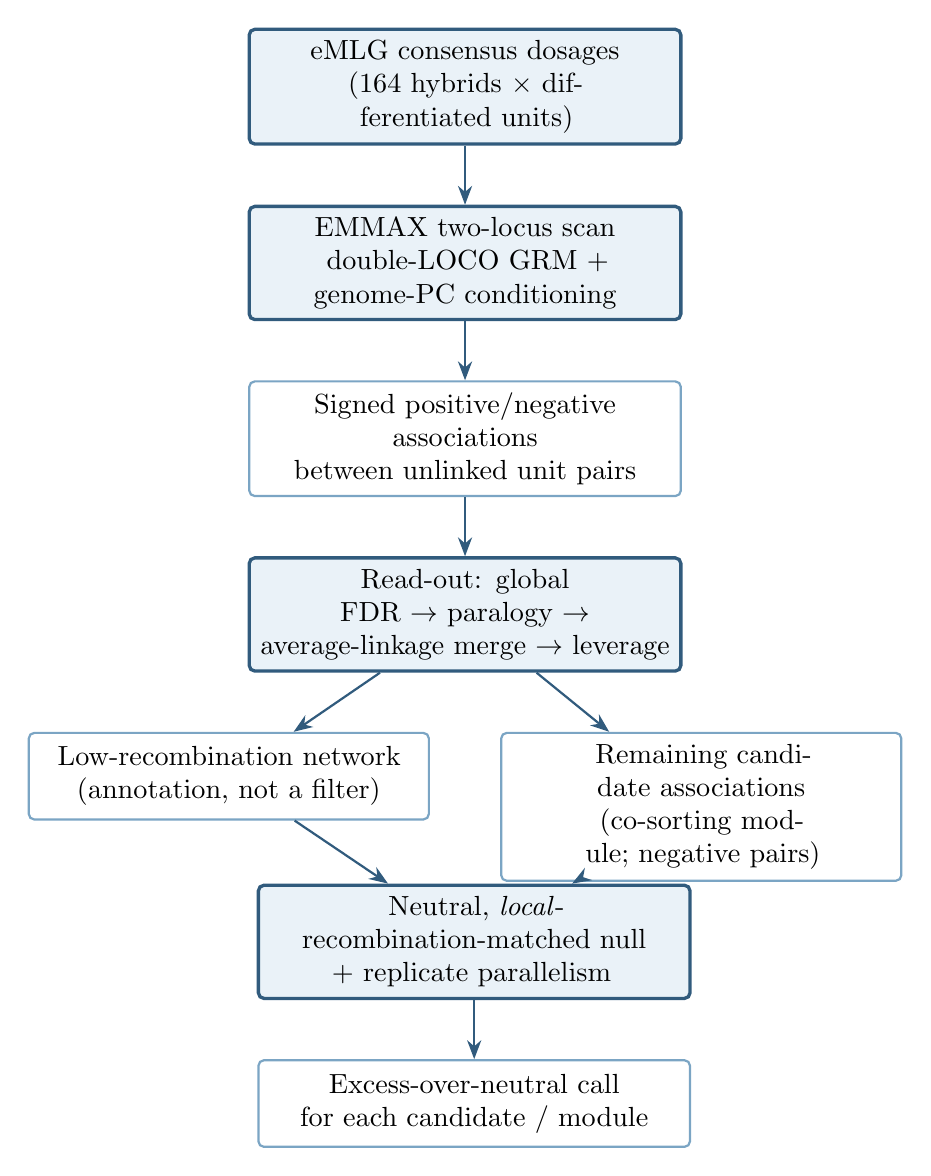
\begin{tikzpicture}[
  node distance=7.5mm and 12mm,
  box/.style={draw=Accent, rounded corners=2pt, very thick, fill=NoteBlue,
    align=center, text width=52mm, minimum height=11mm, inner sep=4pt},
  result/.style={draw=NoteBorder, rounded corners=2pt, thick, fill=white,
    align=center, text width=52mm, minimum height=11mm, inner sep=4pt},
  arrow/.style={-{Stealth[length=2.4mm]}, thick, draw=Accent}
]
\node[box] (units) {eMLG consensus dosages\\(164 hybrids $\times$ differentiated units)};
\node[box, below=of units] (scan) {EMMAX two-locus scan\\double-LOCO GRM $+$ genome-PC conditioning};
\node[result, below=of scan] (tests) {Signed positive/negative associations\\between unlinked unit pairs};
\node[box, below=of tests] (filter) {Read-out: global FDR $\to$ paralogy $\to$\\average-linkage merge $\to$ leverage};
\node[result, below=of filter, xshift=-30mm, text width=48mm] (struct)
  {Low-recombination network\\(annotation, not a filter)};
\node[result, below=of filter, xshift=30mm, text width=48mm] (cand)
  {Remaining candidate associations\\(co-sorting module; negative pairs)};
\node[box, below right=8mm and -22mm of struct] (null)
  {Neutral, \emph{local}-recombination-matched null\\$+$ replicate parallelism};
\node[result, below=of null] (call) {Excess-over-neutral call\\for each candidate / module};

\draw[arrow] (units) -- (scan);
\draw[arrow] (scan) -- (tests);
\draw[arrow] (tests) -- (filter);
\draw[arrow] (filter) -- (struct);
\draw[arrow] (filter) -- (cand);
\draw[arrow] (struct) -- (null);
\draw[arrow] (cand) -- (null);
\draw[arrow] (null) -- (call);
\end{tikzpicture}
\caption{\textbf{Analytical workflow for the intrinsic arm.} A single
structure-corrected scan is summarized by one procedure into a
low-recombination co-ancestry network and a short candidate list. Low recombination is
annotated, never used to discard loci; every unit is carried into the neutral,
local-recombination-matched null that provides the final call.}
\label{figD:workflow}
\end{figure}
\clearpage

\section{Units, orientation, and the unlinked definition}\label{sec:units}

The analytical unit is the eMLG consensus dosage of an LD cluster (continuous, on an
\Faq-oriented $0$--$2$ scale; no hard-calling), restricted to the parent-differentiated
units used as informative markers throughout. Consensus orientation and the parental gate
(pooled parental MAF $\geq0.15$) follow the companion methods, so that a unit's dosage and
its diagnostic index (DI) are on consistent scales.

Two units were treated as \emph{unlinked} when they lay on different chromosomes, or on the
same chromosome more than $\mathrm{LINK}_{\mathrm{cM}}=10$~cM apart on the genetic map.
At the recombination rates of this genome, 10~cM corresponds to approximately 99\% decay of
admixture LD over the estimated $\sim$50 generations since contact. Per-unit map positions
were calculated as the median positions of their member markers. The 10-cM criterion is a
deliberately conservative threshold for this association screen and is distinct from the
0.5-cM merge limit used to construct the LD-reduced units.

\section{Structure-corrected two-locus association (EMMAX)}\label{sec:emmax}

\subsection{Rationale and model}

To ask whether two units are associated \emph{beyond} what shared ancestry and relatedness
predict, we treat one unit's consensus dosage as a quantitative trait and test its
association against every other differentiated unit in a linear mixed model,
\begin{equation}
  y_i = \mu + \beta\,x_j + u + \varepsilon,\qquad
  u\sim N(0,\sigma_g^2 K),\quad \varepsilon\sim N(0,\sigma_e^2 I),
  \label{eq:emmax}
\end{equation}
where $y_i$ is the focal unit's dosage across the 164 individuals, $x_j$ a candidate
partner, and $K$ a genomic-relationship matrix (EMMAX; Li, Kemppainen, Rastas \& Meril\"a).
This is a genome scan in which the ``phenotype'' is one unit and the ``markers'' are all the
others; variance components are estimated once under the null and reused for every partner.

\subsection{Controlling for ancestry and relatedness}

The genomic-relationship matrix captures broad genetic structure and relatedness among
individuals. In addition, each focal dosage was adjusted for the first ten genetic principal
components. Three model choices were used:
\begin{enumerate}
  \item \textbf{Relationship matrix.} $K$ was built from differentiated units because these
        units capture the ancestry variation most relevant to the scan. A matrix based on a
        neutral background produced residual test-statistic inflation.
  \item \textbf{Double leave-one-chromosome-out.} Because the scan is symmetric, both the
        focal and the partner chromosome are dropped from $K$, so neither tested unit's own
        region deflates its association. This keeps the test calibrated ($\lambda\approx
        0.98$--$1.05$; Fig.~\ref{figD:emmax}).
  \item \textbf{Genetic-PC adjustment.} Each focal dosage was adjusted for the first ten
        principal components calculated from the differentiated eMLGs. This reduced residual
        associations with secondary axes of genetic structure.
\end{enumerate}
Each association is signed by its structure-corrected generalised-least-squares coefficient
(positive or coupling, $+$; negative or repulsion, $-$). The targeted scan
scanned 51 focal units (bidirectional candidates, extreme among-population-covariance units,
and controls including a random-focal set for calibration).

False-discovery rates therefore refer to all comparisons in this targeted screen, not to an
unbiased genome-wide sample of focal regions.

\begin{figure}[t]
\centering
\includegraphics[width=\textwidth]{../Figures/moduleD_emmax_writeup.png}
\caption{\textbf{Calibration and read-out of the structure-corrected scan.} Diagnostic
summary of the double-LOCO, genome-PC-conditioned EMMAX scan: quantile--quantile calibration
of the association statistic ($\lambda\approx0.98$--$1.05$), an example focal Manhattan with
its self-locus and linked block removed, and the signed positive and negative associations. The
scan is calibrated and its strongest associations are cross-chromosome, motivating the
paralogy filter of Section~\ref{sec:paralogy}.}
\label{figD:emmax}
\end{figure}

\section{Cross-chromosome paralogy}\label{sec:paralogy}

Duplicate sequence or incorrect mapping can produce nearly identical genotypes at different
assembly locations. Such pairs cannot be removed using genetic distance. We therefore
calculated the correlation between each pair's consensus dosages within each population and
used the median absolute correlation across populations. Pairs with median
$|r|>\mathrm{PARALOGY}_r=0.9$ were flagged as potential duplicate or mismapped regions.
Genotype concordance and excess observed heterozygosity were used as supporting diagnostics
(Fig.~\ref{figD:paralogy}). These criteria identify candidate technical artefacts rather than
proving paralogy.

\begin{figure}[t]
\centering
\includegraphics[width=\textwidth]{../Figures/moduleD_paralogy_writeup.png}
\caption{\textbf{The paralogy discriminant.} Distribution of median within-population $|r|$
for unlinked pairs, with the $0.9$ flag; the corroborating rise in genotype concordance and
per-unit excess heterozygosity toward $|r|=1$; and the separation of flagged (technical) from
retained (candidate) pairs. Distance filtering is orthogonal to this signal-based filter, so
both are applied.}
\label{figD:paralogy}
\end{figure}

\section{Filtering and network summarization}\label{sec:readout}

The scan was read out by one procedure rather than per-focal thresholds, so that the
structural and pair-specific components separate under a single criterion.

\begin{enumerate}
  \item \textbf{False-discovery control.} All unlinked focal--partner tests
        ($1.38\times10^{6}$) were pooled and controlled at a global Benjamini--Hochberg
        $q<Q_{\mathrm{FDR}}=0.01$ across the targeted screen.
  \item \textbf{Paralogy filter} (Section~\ref{sec:paralogy}).
  \item \textbf{Regional consolidation.} For this network only, correlated units on the same
        chromosome and within 10~cM were combined by average-linkage clustering
        ($|r|>\mathrm{MERGE}_r=0.5$). This prevented one extended region from being counted as
        several interacting loci.
  \item \textbf{Leave-one-population-out robustness.} An edge was retained only if its
        among-population allele-frequency correlation survived leave-one-population-out
        analysis ($\min_k|r_{-k}|\geq\mathrm{LEV}_{\mathrm{LOO}}=0.3$).
\end{enumerate}

Cross-chromosome correlation \emph{modules} were then defined by average-linkage clustering
of the meta-node consensuses \emph{across} chromosomes, cut at $|r|>\mathrm{MODULE}_r=0.4$.
Unlike the within-chromosome merge, this groups co-varying regions genome-wide. These modules
were used as descriptive summaries and for genotype visualization.

\section{Recombination annotation, not a filter}\label{sec:recomb}

Each meta-node was annotated by its recombination percentile relative to the differentiated
background. Units below the tenth percentile
($\mathrm{STRUCT}_{\mathrm{pct}}=0.10$) were labelled low-recombination regions. This was a
descriptive annotation rather than an exclusion criterion. Low recombination can preserve
long ancestry blocks and can also contribute to the maintenance of coadapted variation;
consequently, it does not by itself distinguish neutral from selective explanations.

\section{Neutral comparison}\label{sec:null}

The empirical scan cannot determine whether the retained associations exceed expectations
under neutral admixture. This requires applying the same scan to simulations generated on
the empirical recombination map, with comparable ancestry, sampling, and population history.
Observed pairs and modules can then be compared with simulated regions experiencing similar
local recombination. Until that comparison is complete, the retained associations are treated
as exploratory candidates rather than inferred incompatibilities.

\section{Statistical interpretation}\label{sec:interp}

The analyses are conditional on the sampled populations, quality filters, and targeted focal
set. The mixed model reduces covariance associated with ancestry and relatedness but cannot
guarantee that all structure has been removed. Low recombination is used as context rather
than evidence for either neutrality or selection. No pair is called an incompatibility on the
basis of this association screen alone; retained associations require comparison with the
neutral simulations and independent biological scrutiny.

\begin{longtable}{>{\raggedright\arraybackslash}p{0.24\textwidth}
                  >{\raggedright\arraybackslash}p{0.40\textwidth}
                  >{\raggedright\arraybackslash}p{0.25\textwidth}}
\caption{Principal parameter settings for the intrinsic (two-locus) arm.}
\label{tabD:parameters}\\
\toprule
Analysis & Parameter & Value \\
\midrule
\endfirsthead
\toprule
Analysis & Parameter & Value \\
\midrule
\endhead
Units & Analytical unit & eMLG consensus dosage (differentiated) \\
      & Parental MAF gate & $\geq0.15$ \\
\midrule
Unlinked & Genetic-distance rule & different chr, or same chr $>10$~cM \\
\midrule
EMMAX & Model & LMM, one unit as trait vs all others \\
      & Genomic-relationship matrix $K$ & VanRaden, differentiated units \\
      & Leave-one-out & double (focal $+$ partner chromosome) \\
      & Genome-PC conditioning & top 10 PCs residualised from the focal \\
      & Sign & structure-corrected GLS coefficient \\
      & Calibration & $\lambda\approx0.98$--$1.05$ \\
\midrule
Paralogy & Discriminant & median within-population $|r|$ \\
         & Flag threshold & $>0.9$ \\
\midrule
Read-out & Multiple testing & Benjamini--Hochberg $q<0.01$ across targeted scan \\
         & Regional consolidation & average linkage, $|r|>0.5$, $\leq10$~cM \\
         & Leverage & leave-one-population-out $|r|\geq0.3$ \\
         & Modules & average linkage across chr, $|r|>0.4$ \\
\midrule
Annotation & Low-recombination label (not a filter) & recombination percentile $<0.10$ \\
\midrule
Neutral comparison & Matching & local recombination (real map) \\
                & Corroboration & replicate-population parallelism \\
\bottomrule
\end{longtable}

\begin{thebibliography}{2}
\bibitem{kang2010}
Kang HM, Sul JH, Service SK, Zaitlen NA, Kong S-Y, Freimer NB, Sabatti C, Eskin E.
Variance component model to account for sample structure in genome-wide association studies.
\textit{Nature Genetics}. 2010;42:348--354.
\bibitem{nouhaud2022}
Nouhaud P, Martin SH, Portinha B, Sousa VC, Kulmuni J. Rapid and predictable genome evolution
across three hybrid ant populations. \textit{PLoS Biology}. 2022;20:e3001914.
\href{https://doi.org/10.1371/journal.pbio.3001914}{doi:10.1371/journal.pbio.3001914}.
\end{thebibliography}

\end{document}
